\section{Case Study: Dokobit}

\subsection{About}

Dokobit \cite{dokobit}, trademark and subsidiary of Estina \cite{euipo-dokobit}, offers two products: Document Signing Portal and API solutions.

The first product, the Document Signing Portal, was released in 2014 \cite{dokobit-aboutus}. The primary purpose of this solution is to allow users to upload documents and digitally sign them online.

Estina has acquired the DigiDoc portal (\url{https://digidoc.ee}) from SK ID Solutions in 2016 \cite{sk-digidocacquired} which had the exact purpose. This portal should not be confused with the similarly named DigiDoc4 client Estonians commonly use to sign documents \cite{ria-idee}.

The second product, API solutions, targets businesses in a variety of scopes: signature collection, signing, identification, sealing, and TSP monitoring \cite{dokobit}. In the thesis, we will only consider the Identification service.

Dokobit's Identification service allows Lithuanian, Latvian, Estonian, Finnish, Norwegian, Icelandic, Polish, Belgian, Portuguese, Spanish, and Italian \cite{dokobit} users to authenticate themselves with their countries' scheme.

The company has received ISO/IEC 27001:2013 certification \cite{dokobit-certification} and in 2020 was included in the EU Trusted Service List \cite{eu-trustservices, dokobit-aboutus}, thus it becoming a Qualified Trust Service Provider.

In 2021, the Norwegian electronic identity solutions provider company Signicat AS acquired UAB Dokobit.

\subsubsection{Dokobit Identification Service}

Identification service supports two distinct data flows: Gateway and API. The core difference between them is that the Gateway uses a prebuilt UI on their server. In contrast, the API requires the companies to develop their UI and have their server communicate with Dokobit servers instead. This difference only affects the user experience.

The main advantage of Identity Gateway over Identity API is the added brand trust. A study finds that users "associate higher security feelings with a higher level of brand trust" \cite{ha2004factors}. If an organization has not matured yet as a brand (such as a recent startup), it will make more sense for them to choose Identity Gateway over API. On the contrary, if they are a large, highly trusted organization, such as a bank, it would make more sense to use Identity API and have all user interactions happen on the same domain.

For this thesis, we will only analyze the Identity Gateway.

\paragraph{Embed or Redirect}

Identity Gateway comes in two primary user flows: embedded and redirect-based.

In embedded flow, users could stay on the website, authenticate in a pop-up window, and update the website view accordingly after finishing the authentication process. Embedded flow has the advantage of not requiring the users to leave the website, which is helpful to preserve user data in complex forms.

In redirect-based flow, users are sent to an external website, perform authentication, and redirected back to the company website, in a flow similar to OAuth2.0.

Ultimately, experts consider the embedded flow to be the weaker of the two methods \cite{auth0-universal-vs-embedded} for two main reasons:

\begin{enumerate}
  \item Cross-origin requests are inherently more dangerous, allowing for MitM and CSRF attacks;
  \item The client application, even when embedded, receives full client credentials, which adds another point of compromise in the form of XSS;
\end{enumerate}

When using federated log-in for Native Apps, "best current practice requires that native apps MUST NOT use embedded user-agents to perform authorization requests" \cite{rfc8252}. This practice means that companies who have a mobile app or would consider having one in the future mustn't use the embedded flow.

\subsection{Data Flow}

This section will analyze Dokobit Identity Gateway, redirect-based user flow. The general overview of which can be seen in figure \ref{fig:dokobit-identitygw-redirect}. We can group the authentication process into three parts: establishing a session with Dokobit, user authentication with an eID provider, and user information retrieval.

\begin{figure}
  \centering
  \begin{sequencediagram}
    \newthread{A}{Actor}{}
    \newinst[2]{B}{AuthServer}{}

    \newinst[1]{C}{IDGW Backend}{}
    \newinst[1]{D}{IDGW Frontend}{}

    \begin{call}{A}{1. login()}{B}{3xx Redirect}
      \begin{call}{B}{2. POST /api/authentication/create}{C}{session\_token}\end{call}
    \end{call}
    \begin{call}{A}{3. authorize() [session\_token]}{D}{Auth Page}\end{call}
    \begin{call}{A}{4. login()}{D}{3xx Redirect + [session\_token]}\end{call}
    \begin{call}{A}{5. loginCallback()}{B}{Auth token}
      \begin{call}{B}{6. GET /api/authentication/\{session\_token\}/status}{C}{User data}\end{call}
    \end{call}

  \end{sequencediagram}
  \caption{Dokobit Identity Gateway - Redirect-based user flow \cite{dokobit-idgw-docs}}
  \label{fig:dokobit-identitygw-redirect}
\end{figure}

\paragraph{Establishing a session with Dokobit}

When a user requests to authenticate, the company's back-end systems' first step is to establish a session with Dokobit Identity Gateway. To do this, a {POST} request must be made to the {/api/authenticate/create} endpoint. This response will contain the session identifier and the redirect URL. Users will have to go there to interface with their eID providers.

Sample HTTP request data can be seen in listing \ref{lst:dokobit-challenge-http}.

\begin{lstlisting}[caption={Handling Dokobit session creation}, label={lst:dokobit-challenge-http}]
  Request:
  POST https://id-sandbox.dokobit.com/api/authentication/create?access_token=YOUR_ACCESS_TOKEN
  {
      'return_url': 'https://id-sandbox.dokobit.com/example/success.php'
  }
  
  Response:
  {
    "status": "ok",
    "session_token": "02f922c9917231ea8acbbbcf63796924af548c801d75772f2b1701b413462c61",
    "url": "https://id-sandbox.dokobit.com/auth/02f922c9917231ea8acbbbcf63796924af548c801d75772f2b1701b413462c61",
    "expires_in": 3600
  }
\end{lstlisting}

\paragraph{User authentication with an eID provider}

After the back-end successfully creates a session, they must redirect the user to the received endpoint. An easy way to accomplish that is to respond to the initial authentication request with HTTP status 302 - Found.

Most of the heavy lifting with authentication is delegated to this step and handled by Dokobit. The company's back-end systems should wait for the user to return after authenticating.

\paragraph{User information retrieval}

After the user returns after successful authentication, the back-end servers should make a {GET} request to {/api/authentication/session\_token/status} endpoint. The company can securely receive the user information via a backchannel.

Sample HTTP request data can be seen in listing \ref{lst:dokobit-handleremote-http}.

\begin{lstlisting}[caption={Handling Dokobit session creation}, label={lst:dokobit-handleremote-http}]
  Request:
  GET https://id-sandbox.dokobit.com/api/authentication/SESSION_TOKEN/status?access_token=YOUR_ACCESS_TOKEN
  
  Response:
  {
      "status": "ok",
      "certificate": { ... },
      "code": "30303039914",
      "country_code": "lt",
      "name": "DEMO",
      "surname": "SMART-ID",
      "authentication_method": "smartid",
      "date_authenticated": "2019-05-06T12:15:34+03:00"
  }
\end{lstlisting}

\subsection{Trust Anchor}

Dokobit assumes the role of being the trust anchor. This means that it also acts as a single point of failure. Should Dokobit become compromised, all applications using Dokobit will become susceptible to impersonation. On the flip side, there is only one system company developers need to implement, meaning that it would be harder for adversaries to break into the system via external means.

Companies should consider the risks when using a provider capable of dictating who the person is, as no integrity checks are supported in the protocol.

From a technical aspect, these risks aren't much different from those applicable to the eeID service.

\subsection{Pricing}

Dokobit is a commercial product, and therefore it has associated usage costs. In 2022, these costs are as seen in the table \ref{tab:dokobit-pricing}.

\begin{table}[h]
  \centering
  \caption{Dokobit Identity Gateway pricing 2022}
  \begin{tabular}{| l | l | l | l |}
    \hline
    \bf{Plan} & \bf{Number of transactions} & \bf{Monthly fee} & \bf{Price per extra transaction} \\
    \hline
    1         & 700                         & 50 €             & 0,071 €                          \\
    \hline
    2         & 1 600                       & 100 €            & 0,063 €                          \\
    \hline
    3         & 5 000                       & 250 €            & 0,050 €                          \\
    \hline
    4         & 12 000                      & 500 €            & 0,042 €                          \\
    \hline
  \end{tabular}
  \label{tab:dokobit-pricing}
\end{table}

Each pricing tier includes a specific number of transactions and adds a cost for each transaction exceeding it. For example, if the total amount of transactions is 200, the price will still be 50 €, as the number of transactions has not reached 700.

Assuming the company's users authenticate around 25 times per month, the monthly user price will be in the ballpark of 1-2 €.

\subsection{Security Requirements}

Of the three case studies analyzed in the thesis, Dokobit Identity Gateway was the only one that did not provide any validation requirements to the relying party, only a single integration example \cite{dokobit-idgw-docs}. This flow, however, is very similar to the one used by the eeID service and will be analyzed with the same best practices document \cite{ietf-oauth-security-topics-19}.

\paragraph{Communication channel}

The Dokobit identity gateway uses a secure communication channel, encrypted end-to-end using HTTPS. When the system is integrated correctly, malicious clients (or user agents) have no possible way of influencing any of the authentication parameters without triggering alarms when validating the request.

\subsubsection{Protocol's built-in security features}

\paragraph{Replay attacks}

\begin{itemize}
  \item Identity Gateway will reject the second GET request with the session id.
\end{itemize}

The developer does not have to implement state management to verify that a given session token was used only once. Mitigation measures are sufficient.

\paragraph{Insufficient Redirect URI Validation}

\begin{itemize}
  \item The adversary does not have any agency over redirect URI after authentication, as the {authorize} endpoint does not have any query parameters.
  \item The redirect\_url parameter when sending the initial request outlined in step 3 of the sequence diagram cannot be longer than 255 ASCII characters.
  \item The redirect URL is never validated on the Dokobit servers, as it was never registered as a client. Each redirect URL is generated for one-time use.
\end{itemize}

Adversaries cannot influence the redirect URI. If companies use a static redirect URL, mitigation measures are sufficient.

\subparagraph{Credential Leakage via Referrer Headers}

\begin{itemize}
  \item Dokobit Identity Gateway does not include third-party resources (javascript, image, or other); therefore, it cannot leak the session token.
  \item The company is required not to have any third-party resources on the authentication and redirect pages.
\end{itemize}

Dokobit does not leak credentials via Referrer Headers. The developers should not embed third-party resources in the critical authentication pages (all resources used in their service are from their domain, see figure \ref{fig:dokobit-leakviareferrer}). Mitigation measures are sufficient.

\begin{figure}
  \centering
  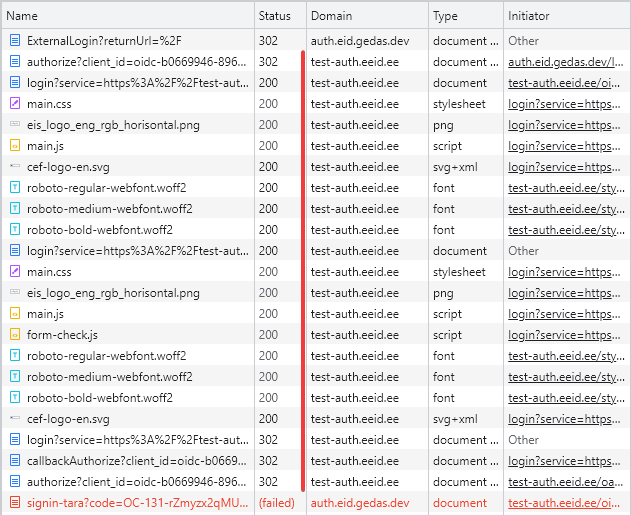
\includegraphics[scale=0.6]{dokobit/leakviareferrer}
  \caption{The Dokobit Identity Gateway does not use resources outside of their domain in the authentication flow}
  \label{fig:dokobit-leakviareferrer}
\end{figure}

\subparagraph{Credential Leakage via Browser History}

\begin{itemize}
  \item Session ids are stored in browser history (see figure \ref{fig:dokobit-leakviahistory}); however, they are single-use only and are immune to replay attacks.
\end{itemize}

The only thing adversaries could extract from the browser history is a used-up session-id, which does not provide much value with sufficient CSRF measures. Mitigation measures are adequate.

\begin{figure}
  \centering
  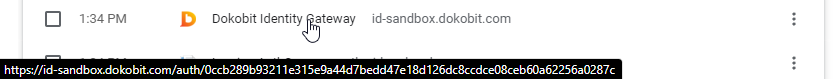
\includegraphics[scale=0.6]{dokobit/leakviahistory}
  \caption{Session id is leaked inside the browser history when using Dokobit authentication}
  \label{fig:dokobit-leakviahistory}
\end{figure}

\subparagraph{Session Token Injection and Cross-Site Request Forgery}

Adversaries would perform the injection and CSRF attacks identically.

\begin{itemize}
  \item The protocol does not protect against session token injection attacks.
  \item The protocol also adds more attack surfaces by issuing the session token before the user signs in, allowing the adversary to obtain or inject it before and after the user performs authentication.
  \item It is possible to mitigate adversaries stealing a victim's session.
  \item \textbf{It is impossible to mitigate adversaries injecting their session} (phishing).
\end{itemize}

Identity Gateway protocol does not have security measures built-in against session token injection or CSRF attacks. It is possible to prevent adversaries from being able to redeem the victim's session. However, there is \textbf{no possible way to prevent adversaries from injecting their Dokobit session}.

From the attacker's point of view, they can exploit this vulnerability by performing these steps \cite{video-exploitdokobit}:

\begin{enumerate}
  \item Establish session with identity server and Dokobit;
  \item Trick the user into opening the link issued by Dokobit;
  \item After the user authenticates, but before gets redirected, reload the page;
  \item If an adversary managed to do it in time, they receive that person's access;
\end{enumerate}

The only way to mitigate this attack for the user will be to make the authentication server invalidate the authenticated session if a request presents the same session\_id. Thankfully, it is easy to detect if the server has consumed the session token already, as Dokobit would reject additional HTTP requests, as described in replay attack mitigation.

Mitigation measures are \textbf{weak}, as the Dokobit's internal log-in page is susceptible to CSRF attacks, and developers should be ready to implement authentication session revocation.

\subparagraph{Clickjacking}

\begin{itemize}
  \item Dokobit auth page does not use Content-Security-Policy. However, it does use header X-Frame-Option: {SAMEORIGIN} (see figure \ref{fig:dokobit-responseheaders}).
  \item The sameorigin feature is used in conjunction with CORS to support embedded flow, however it would be better if Frame Options were outright disabled.
  \item Relying party should integrate this or a similar countermeasure.
\end{itemize}

Mitigation measures are sufficient on almost all browsers released in the last ten years \cite{caniuse-xframeoptions}.

\begin{figure}
  \centering
  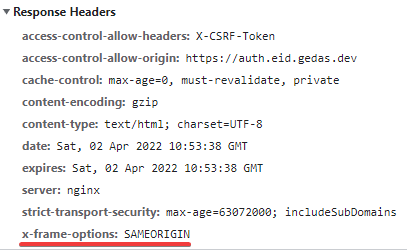
\includegraphics[scale=0.7]{dokobit/frameoptions}
  \caption{Response headers browsers receive when opening the eeID service's login page}
  \label{fig:dokobit-responseheaders}
\end{figure}

\subsubsection{Validation requirements for the relying party}

In the previous section, we saw the security features of the protocol. The relying party should implement validation and reject requests for some of the features if those validations do not match. This section will contain all of the features the RP needs to address.

\paragraph{Misconfiguration Attacks}

\subparagraph{Incorrect URL specified}

The relying party should make sure to use the correct Dokobit Identity Gateway endpoints. For test environment the URL is \url{https://id-sandbox.dokobit.com}, and for production - \url{https://id.dokobit.com}. A connection with a malicious party could be established when using the incorrect URL.

Developers should make sure these values are not easily editable (such as placed in environment variables) by anyone. Best they should be hardcoded in the application.

\subparagraph{Weak TLS configuration}

TLS is the primary defense mechanism against MitM attacks when connecting to the Dokobit servers. WorkAuth's IT Ops team should ensure that the server does not trust any malicious CA.

\paragraph{Session Token Injection and Cross-Site Request Forgery}

Like in the eeID service, the primary validation user has to implement is protection against CSRF and code injection. Developers can accomplish this by binding the dokobit session\_id to the user agent session.

\subparagraph{Attack description}

For reference to how the mitigation works, we will use the figure \ref{fig:dokobit-identitygw-redirect}. We will provide two examples for the countermeasure: without and with session binding.

Our attack exists right before the final redirect (right before step 5 in the figure \ref{fig:dokobit-identitygw-redirect}). Unlike in the case with eeID, this protocol has multiple places where an attacker can extract the session\_id as it is generated before the user is redirected, and not after they complete the authentication process. Regardless, an attacker cares about tokens that have been authenticated, but not consumed, which puts us right before step 5.

\subparagraph{Attack \#1 - No binding}

When a subsequent request is made to the authorization endpoint, if the session\_id was authenticated, Dokobit will automatically redirect the user to WorkAuth's identity server and finish the process. Without user agent binding, it is trivial to establish a session.

\subparagraph{Attack \#2 - With user agent binding}

Before WorkAuth's server redirects the user agent to Dokobit's authorization endpoint, it first creates a cookie containing the session\_id in an encrypted form. This value will be used later.

We run the first attack per usual, interrupting the flow in the same place. When the attacker tries to authenticate, the server will successfully decrypt the cookie value. However, the server will fail to match the session\_id and detect the attack.

Because everything is bound to the same session\_id, this one cookie is sufficient to mitigate against both CSRF and code injection attacks.

\subsection{Integration}

Unlike the eeID service, no libraries exist for Dokobit Identity Gateway, and users must manually integrate the flow. Fortunately, the integration is very straightforward.

The code snippets \ref{lst:dokobit-challenge} and \ref{lst:dokobit-handleremote} are akin to data flow in figure \ref{fig:dokobit-identitygw-redirect}. Numbers in comments directly correspond to the steps in the flow.

The first code block (listing \ref{lst:dokobit-challenge}) has three main parts:

\begin{enumerate}
  \item establish a session with Dokobit as described in listing \ref{lst:dokobit-challenge-http};
  \item append an \textbf{encrypted} session cookie which would bind the browser to that specific Dokobit session (this cookie stores the encrypted session\_token);
  \item redirect the user to the authorization endpoint;
\end{enumerate}

\begin{lstlisting}[caption={Handling Dokobit session creation}, label={lst:dokobit-challenge}]
  // [1] Login
  protected override async Task HandleChallengeAsync(AuthenticationProperties properties)
  {
      if (string.IsNullOrEmpty(properties.RedirectUri))
          properties.RedirectUri = OriginalPathBase + OriginalPath + Request.QueryString;

      // [2] Establish session with Dokobit
      var body = JsonSerializer.Serialize(new { return_url = BuildRedirectUri(Options.CallbackPath) });
      var response = await ExecuteRequestAsync(HttpMethod.Post, "/api/authentication/create", body);
      response.EnsureSuccessStatusCode();

      using var sessionResponse = await JsonDocument.ParseAsync(await response.Content.ReadAsStreamAsync(Context.RequestAborted));
      var root = sessionResponse.RootElement;

      // Save session token to encrypted cookie properties
      properties.Items["session_token"] = root.GetString("session_token");

      Response.Cookies.Append(Options.StateCookie.Name!, Options.StateDataFormat.Protect(properties), Options.StateCookie.Build(Context, Clock.UtcNow));
      var redirectContext = new RedirectContext<DokobitOptions>(Context, Scheme, Options, properties, root.GetString("url")!);

      // [3] Redirect the user agent
      await Events.RedirectToAuthorizationEndpoint(redirectContext);
  }
\end{lstlisting}

After the user authenticates and returns, the next code block gets executed (listing \ref{lst:dokobit-handleremote}). This code performs request validation in addition to retrieving the user data:

\begin{enumerate}
  \item try to decrypt the cookie data - if decryption fails, it was likely tampered with, and the application cannot proceed with the authentication;
  \item try to obtain the session token from query parameters - it should always exist if the request was not tampered with;
  \item verify that the session\_token received from cookie and query parameters match - this prevents attackers from stealing session tokens;
  \item redeem the session\_token and receive user data as described in listing \ref{lst:dokobit-handleremote-http};
  \item clean up the used cookies;
  \item issue an access token or a new session for use in the company;
\end{enumerate}

\begin{lstlisting}[caption={Handling access token creation}, label={lst:dokobit-handleremote}]
  // [5] Callback
  protected override async Task<HandleRequestResult> HandleRemoteAuthenticateAsync()
  {
      // Decrypt the user agent session. If we fail here, it means that cookie was likely tampered with
      var properties = Options.StateDataFormat.Unprotect(Request.Cookies[Options.StateCookie.Name!]);
      if (properties == null)
          return HandleRequestResult.Fail("Invalid state");
  
      // Verify if session token received matches the one we initially saved
      var sessionToken = Request.Query["session_token"];
      if (StringValues.IsNullOrEmpty(sessionToken))
          return HandleRequestResult.Fail("Missing session_token", properties);
  
      if (properties.Items["session_token"] != sessionToken)
          return HandleRequestResult.Fail("Unexpected session_token received", properties);
  
      // [6] Validation successful, obtain user identity
      var response = await ExecuteRequestAsync(HttpMethod.Get, $"/api/authentication/{sessionToken}/status");
      response.EnsureSuccessStatusCode();
  
      // Cleanup
      Response.Cookies.Delete(Options.StateCookie.Name!);
  
      // Establish an authenticated session
      await using var stream = await response.Content.ReadAsStreamAsync(Context.RequestAborted);
      using var user = await JsonDocument.ParseAsync(stream);
  
      var ticket = await CreateTicketAsync(new ClaimsIdentity(ClaimsIssuer), properties, user.RootElement);
      return HandleRequestResult.Success(ticket);
  }
\end{lstlisting}

After completing these steps, the final code will be resilient to CSRF attacks.

\subsection{Discovered weaknesses}

\subsubsection{API key transferred via query parameters}

\subsubsection{CSRF on the authorize endpoint}

When performing a session token injection attack, relying parties can successfully protect themselves by binding the Dokobit's session token to the user agent session. Unfortunately, this does not prevent attackers from injecting their session tokens into victims' computers.

From the attacker's point of view, they can exploit this exploit can be achieved by performing these steps \cite{video-exploitdokobit}:

\begin{enumerate}
  \item Establish session with identity server and Dokobit;
  \item Trick the user into opening the link issued by Dokobit (phishing works);
  \item After the user authenticates, but before gets redirected, reload the page;
  \item If an attacker manages to achieve it in time, they receive that person's access;
\end{enumerate}

A video exists showing a live demonstration of how this attack appears for both attacker and victim \cite{video-exploitdokobit}.

\paragraph{The underlying issue}

At its core, this exploit is possible because of three issues: 

\begin{enumerate}
  \item The attacker knows the response session token. Because all requests are correlated with the same session token, the attacker already knows the redirect URL.
  \item Nothing is binding the authentication and redirect processes.
  \item Requests automatically redirect the user to the final endpoint after authentication if the session token was not yet consumed.
\end{enumerate}

The third point is fascinating, as it glues issues 1 and 2 together. We can see how it connects these issues by looking at an authentication example (see figure \ref{fig:dokobit-vuln-csrf}).

\begin{figure}
  \centering
  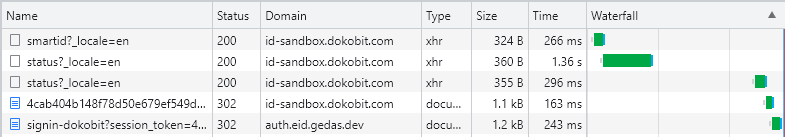
\includegraphics[scale=0.7]{dokobit/vuln_csrf}
  \caption{Waterfall of Dokobit Smart-ID authentication}
  \label{fig:dokobit-vuln-csrf}
\end{figure}

We need to look at the waterfall diagram of the requests Identity Gateway makes to see why this attack works. The first request ({smartid}) starts a background task to authenticate with Smart-ID. Second and third requests ({status}) check on that background job and complete the request after it does. Notably, the checks are done with a delay, meaning there could be some amount of time (around one second) when the authentication process is finished, but the browser is not aware of it.

When the page is refreshed, status checks are done immediately, so if an attacker managed to refresh the page in the short 1-second window, they would steal the session. Ironically, if the WorkAuth developers were diligent enough to prevent CSRF attacks, in the server's eyes, the victim would be seen as an attacker, and their request would be rejected, giving even more time for attackers to exchange the token.

There may be some band-aid solutions for this exploit, but we see only one true fix: bind the Smart-ID (and other) authentication schemes to the current request or make it synchronous. Regular CSRF countermeasures are sufficient (generating a token on the page and using it to the end).

\paragraph{Disclosure}

\begin{itemize}
  \item Mar 21, 2022: Informed Dokobit CIRT about the exploit.
  \item Mar 27, 2022: Dokobit CIRT acknowledged the issue and started to work on a fix.
\end{itemize}